\newpage
\section{Implementazione}


\subsection{Francesco Foschini}
Il mio compito all'interno del progetto, è stato quello di modellare la gerarchia di \texttt{Entity} del gioco.
In particolare mi sono occupato della implementazione del model degli Zombie, dei proiettili e l'attore definisce il comportamento dei proiettili.
Ho partecipato inoltre allo sviluppo del Troop Actor del Menù Screen e del GameScreen.

\subsubsection{Bullet}
I proiettili rappresentano all'interno del gioco l'attacco delle piante e degli zombie che viene sparato dalle torri
per infliggere danni. Grazie alla buona gerarchia di caratteristiche definite in \texttt{Entity}, è stato possibile grazie  ai \textbf{mixin}
dotare il trait \texttt{Bullet} dell'abilità di movimento (\texttt{Movement Ability}).
Il trait Bullet rappresenta quindi l'entità base "sparata" da una Troop.
Tutti i bullet presentano un comportamento comune: possiedono una posizione, una velocità, una dimensione ed un danno.


Successivamente a una prima versione dei Bullet ho pensato di rifattorizzare i Bullet individuando due diversi sottotipi: \texttt{ZombieBullet} e \texttt{PlantBullet}.
Il primo è un trait che modella l'attacco base degli zombie mentre il secondo si riferisce all'attacco delle piante.
Attraverso il metodo checkCollision i PlantBullet possono collidere solamente contro le entità di tipo Zombie mentre,
al contrario, gli ZombieBullet potranno colpire solamente le entità sottotipo di Plant.
Mi sono successivamente concentrato nell'implementazione di due tipi di ZombieBullet: PawBullet (il bullet dei
BasicZombie e FastZombie) e lo SwordBullet(il bullet dei WarriorZombie).
Lo SwordBullet è un attacco molto più potente rispetto al PawBullet.

Volendo seguire un approccio puramente funzionale, favorendo l'immutabilità delle entità, il metodo di
aggiornamento della posizione di un bullet deve creare un nuovo bullet con la nuova posizione.
Questo comportamento è comune a tutti i tipi di bullet: l'aggiornamento di ognuno di questi deve
tornare il tipo di bullet corretto. A tal proposito è stato utilizzato il metodo di scala  \texttt{copy()}.
\textit{copy} può essere utilizzato solo nelle \texttt{case class}, quindi tutte le classi che estendono
\texttt{Bullet} lo utilizzano per restituire un nuovo Bullet con la posizione aggiornata.
Attraverso questa strategia l'aggiornamento della posizione dei bullet può essere effettua utilizzando la \textbf{infix notation}:
\begin{verbatim}
    val bullet = Bullets.ofType[PawBullet]
    bullet withPosition (0,0)
\end{verbatim}
La stessa soluzione è stata poi adottata anche nelle Troop.

La velocità e il danno di ogni tipo di bullet è definito nell'oggetto BulletDefaultValues.

Per la creazione di ogni tipo di Bullet abbiamo pensato di utilizzare il \textbf{pattern builder}.
Dentro all'object \texttt{Bullets} è stato creato un \texttt{trait BulletBuilder}
con un unico metodo \textit{build} che ritorna un sottotipo di \texttt{Bullet}.
Utilizzando le \textbf{given conversion} sono state definite un'istanza di builder per la creazione di una istanza
di ogni possibile tipo di \texttt{Bullet}.
E' stato, infine, definito un metodo \textit{ofType} che che dato un tipo
di \texttt{Bullet} chiama il builder corretto per restituire la nuova entità.
\begin{verbatim}
    object Bullets:
      /**
       * A builder used to create [[Bullet]].
       *
       * @tparam T The type of the [[Bullet]].
       */
      trait BulletBuilder[B <: Bullet]:
        /**
         * @return A [[Bullet]] of type [[B]]
         */
        def build: B

      /**
       * Given instances to create a [[PeaBullet]].
       */
      given BulletBuilder[PeaBullet] with
        override def build: PeaBullet = PeaBullet()

      /**
       * Given instances to create a [[SnowBullet]].
       */
      given BulletBuilder[SnowBullet] with
        override def build: SnowBullet = SnowBullet()

      /**
       * Given instances to create a [[CherryBullet]].
       */
      given BulletBuilder[CherryBullet] with
        override def build: CherryBullet = CherryBullet()

      /**
       * Given instances to create a [[PawBullet]].
       */
      given BulletBuilder[PawBullet] with
        override def build: PawBullet = PawBullet()

      /**
       * Given instances to create a [[SwordBullet]].
       */
      given BulletBuilder[SwordBullet] with
        override def build: SwordBullet = SwordBullet()

      /**
       * A DSL method to create every type of [[Bullet]].
       *
       * @param bulletBuilder The [[BulletBuilder]] of the type needed.
       * @tparam B The [[Bullet]] type.
       * @return The [[Bullet]] of the specified type.
       */
      def ofType[B <: Bullet](using bulletBuilder: BulletBuilder[B]): B =
        bulletBuilder.build
\end{verbatim}

Tutto ciò rende più funzionale l'istanziamento di un nuovo Bullet.
Viene mostrato di seguito come istanziare un PawBullet:
\begin{verbatim}
    val bullet = Bullets.ofType[PawBullet]
\end{verbatim}

\begin{figure}[H]
    \centering
    \includegraphics[width=1\linewidth]{img/class-bullet}
    \caption{Diagramma delle classi rappresentante i \texttt{ZombieBullet}.}
    \label{fig:class-bullet}
\end{figure}

Il model del Bullet è stato testato nella classe BulletModelTest

\subsubsection{BulletActor}
Avendo pensato il sistema adottando un'architettura ad attori, abbiamo pensato di incapsulare il comportamento
di ogni proiettile a un \texttt{BulletActor}. Quindi, in fase di creazione, ogni \texttt{Bullet} sarà associato ad un
\texttt{BulletActor} che ne definirà il comportamento.
Il BulletActor ha un solo Behaviour chiamato \texttt{moving}: risponde ai messaggi ricevuti dal GameLoop
Come il TroopActor, ad ogni iterazione del GameLoop il BulletActor riceve un messaggio di \texttt{Update()} a seguito del quale:
\begin{enumerate}
    \item Aggiorna il proprio \texttt{Bullet}.
    \item Manda il suo \texttt{Bullet} aggiornato al GameLoop.
    \item Ricrea il proprio Behaviour con il \texttt{Bullet} aggiornato.
\end{enumerate}
Quando il \texttt{Bullet} collide con un'altra entità riceve un messaggio \texttt{Collision()} a seguito del quale:
\begin{enumerate}
    \item Crea il bullet della propria troop.
    \item Crea un BulletActor che controlla il bullet.
    \item Notifica il GameLoop dell'avvenuta creazione con il messaggio BulletSpawned().

Il comportamento del \texttt{BulletActor} viene mostrato nel seguente diagramma:
\begin{figure}[H]
    \centering
    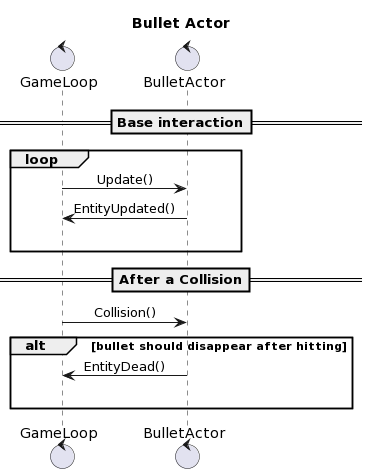
\includegraphics[width=\linewidth]{images/bullet-actor.png}
    \label{Diagramma di sequenza del Troop Actor.}
\end{figure}

Il BulletActor è stato testato nella classe BulletActorTest utilizzando il framework AkkaTest

\subsubsection{Zombie}
Gli Zombie rappresentano una delle entità fondamentali del gioco. In particolare, rappresentano i nemici che l'utente
deve cercare di eliminare attraverso il piazzamento delle piante nel campo di gioco.
Tutti gli zombie sono in grado di muoversi "orrizzontalmente" nelle lane del campo di gioco con una certa velocità: pertanto
attraverso il meccanismo dei mixin il \texttt{trait Zombie} estende il \texttt{trait Troop} a cui aggiunge poi l' abilità \texttt{MovingAbility}.

Quando uno zombie è colpito da un CherryBullet potrebbe essere rallentato, per questo motivo si è deciso di
mettere la velocità in ciascun costruttore per ciascun tipo di zombie implementato.
In questo modo, seguendo un approccio funzionale, quando il CherryBullet collide con uno specifico Zombie
istanzierà nuovamente lo zombie con la velocità aggiornata.
A tal proposito è stata implementata una val \texttt{slowVelocities} dentro all'object ZombieDefaultValues.
E' infatti nell'object \texttt{ZombieDefaultValue} che sono definite tutte le caratteristiche principali per ogni
tipo di Zombie implementato: stato iniziale e di default (\texttt{Moving}), vita iniziale,
il tipo bullet sparato, la velocità di default, la velocità degli Zombie rallentati e un metodo per generare
la posizione iniziale degli zombie.

